\documentclass[12pt]{article}
\usepackage[paper=letterpaper,margin=1.5cm]{geometry}
\usepackage{amsmath}
\usepackage{amssymb}
\usepackage{amsfonts}
\usepackage{mathtools}
%\usepackage[utf8]{inputenc}
%\usepackage{newtxtext, newtxmath}
\usepackage{lmodern}     % set math font to Latin modern math
\usepackage[T1]{fontenc}
\renewcommand\rmdefault{ptm}
%\usepackage{enumitem}
\usepackage[shortlabels]{enumitem}
\usepackage{titling}
\usepackage{graphicx}
\usepackage[colorlinks=true]{hyperref}
\usepackage{setspace}
\usepackage{subfigure} 
\usepackage{braket}
\usepackage{color}
\usepackage{tabularx}
\usepackage[table]{xcolor}
\usepackage{listings}
\usepackage{mathrsfs}
\usepackage{stackengine}
\usepackage{physics}
\usepackage{afterpage}
\usepackage{pdfpages}
\usepackage[export]{adjustbox}
\usepackage{biblatex}

\setstackEOL{\\}

\definecolor{dkgreen}{rgb}{0,0.6,0}
\definecolor{gray}{rgb}{0.5,0.5,0.5}
\definecolor{mauve}{rgb}{0.58,0,0.82}


\lstset{frame=tb,
  language=Python,
  aboveskip=3mm,
  belowskip=3mm,
  showstringspaces=false,
  columns=flexible,
  basicstyle={\small\ttfamily},
  numbers=none,
  numberstyle=\tiny\color{gray},
  keywordstyle=\color{blue},
  commentstyle=\color{dkgreen},
  stringstyle=\color{mauve},
  breaklines=true,
  breakatwhitespace=true,
  tabsize=3
}
\setlength{\droptitle}{-6em}

\makeatletter
% we use \prefix@<level> only if it is defined
\renewcommand{\@seccntformat}[1]{%
  \ifcsname prefix@#1\endcsname
    \csname prefix@#1\endcsname
  \else
    \csname the#1\endcsname\quad
  \fi}
% define \prefix@section
\newcommand\prefix@section{}
\newcommand{\prefix@subsection}{}
\newcommand{\prefix@subsubsection}{}
\renewcommand{\thesubsection}{\arabic{subsection}}
\makeatother
\DeclareMathOperator*{\argmin}{argmin}
\newcommand{\partbreak}{\begin{center}\rule{17.5cm}{2pt}\end{center}}
\newcommand{\alignbreak}{\begin{center}\rule{15cm}{1pt}\end{center}}
\newcommand{\tightalignbreak}{\vspace{-5mm}\alignbreak\vspace{-5mm}}
\newcommand{\hop}{\vspace{1mm}}
\newcommand{\jump}{\vspace{5mm}}
\newcommand{\R}{\mathbb{R}}
\newcommand{\C}{\mathbb{C}}
\newcommand{\N}{\mathbb{N}}
\newcommand{\G}{\mathbb{G}}
\renewcommand{\S}{\mathbb{S}}
\newcommand{\bt}{\textbf}
\newcommand{\xdot}{\dot{x}}
\renewcommand{\star}{^{*}}
\newcommand{\ydot}{\dot{y}}
\newcommand{\lm}{\mathrm{\lambda}}
\renewcommand{\th}{\theta}
\newcommand{\id}{\mathbb{I}}
\newcommand{\si}{\Sigma}
\newcommand{\Si}{\si}
\newcommand{\inv}{^{-1}}
\newcommand{\T}{^\intercal}
\renewcommand{\tr}{\text{tr}}
\newcommand{\ep}{\varepsilon}
\newcommand{\ph}{\varphi}
%\renewcomand{\norm}[1]{\left\lVert#1\right\rVert}
\definecolor{cit}{rgb}{0.05,0.2,0.45}
\addtolength{\jot}{1em}
\newcommand{\solution}[1]{

\noindent{\color{cit}\textbf{Solution:} #1}}

\newcounter{tmpctr}
\newcommand\fancyRoman[1]{%
  \setcounter{tmpctr}{#1}%
  \setbox0=\hbox{\kern0.3pt\textsf{\Roman{tmpctr}}}%
  \setstackgap{S}{-.9pt}%
  \Shortstack{\rule{\dimexpr\wd0+.1ex}{.9pt}\\\copy0\\
              \rule{\dimexpr\wd0+.1ex}{.9pt}}%
}

\newcommand{\Id}{\fancyRoman{2}}
\addbibresource{citations.bib}


% Enter the specific assignment number and topic of that assignment below, and replace "Your Name" with your actual name.
\title{STAT 31020: Homework 4}
\author{Caleb Derrickson}
\date{January 31, 2024}

\begin{document}
\onehalfspacing
\maketitle
\allowdisplaybreaks
\tableofcontents

\newpage
\section{Problem 1}
We aim to understand both trust-region approaches and sparsity of matrices. 
\subsection{Problem 1, part 1}
For the Rosenbrock function of order n we used in last homework,\\
$f(x) = \sum_{i = 1}^{n - 1} \left[ 100 (x_{i+1} - x_i^2)^2 + (x_i - 1)^2\right]$
implement a function to return the sparse Hessian.
\partbreak
\begin{solution}

    I have just added the condition that the returned hessian is sparse. I passed the dense matrix to the sparse() function provided by Matlab.
\end{solution}

\newpage
\subsection{Problem 1, part 2}
We will experiment with sparse and dense linear algebra. Let $b \in \R^n$ be a vector of ones of dimension n. Compute the Hessian $H$ at the point of all entries being equal to 2. Solve the equation $Hx = b$ and time it for $H$ being sparse format and denote the time by a(n) with dense format and denote the time by b(n) using the backslash operator. Plot a(n) and b(n) as functions of n. what seems to be the rough behavior of a(n) and b(n)? 
\partbreak
\begin{solution}

    The plot is given as Figure \ref{fig:MatMult}. I tried fitting polynomials to both plots and I got that the dense matrix time scales roughly by $n^2$ (the coefficient of $n^3$ is of the order $10^{-11}$; for $n^2$, $10^{-8}$), while the sparse matrix scales roughly by $n$ (the coefficient of $n^2$ is of order $10^{-10}$; for $n$, $10^{-7}$). I have been told that I will not see the $n^3$ dominance come into play for such small dimension values in the case of the dense matrix. The way I was constructing my Hessian, I had a nested for loop which really dropped computation time. 
\end{solution}
\vspace{4cm}
\begin{figure}[!h]
    \centering
    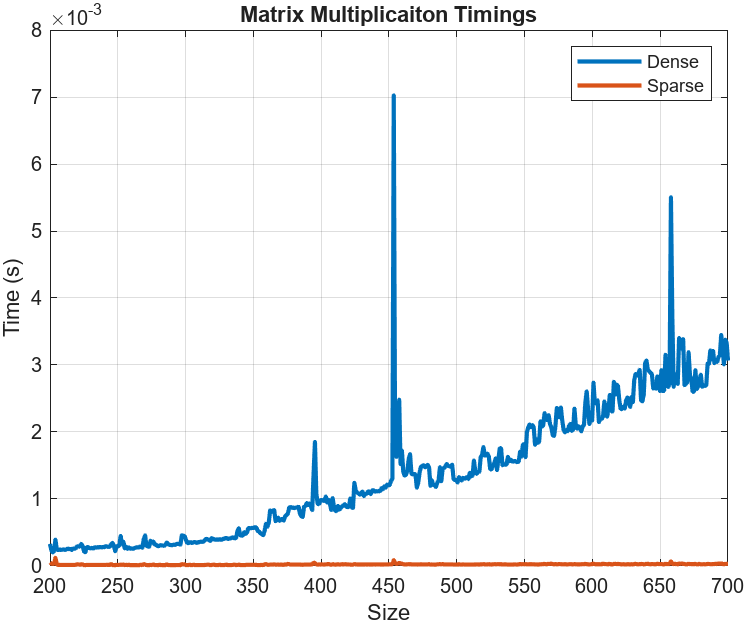
\includegraphics[width = 0.5\textwidth]{Plots/MatrixMultiplicationTimings.png}
    \caption{Solving $Ax = b$ for $A$ dense vs sparse and the given Hessian.}
    \label{fig:MatMult}
\end{figure}

\newpage
\subsection{Problem 1, part 3}
Write a program that implements the dogleg trust-region approach. Experiment with the parameters or by designing your own rules. Report the total number of linear systems solved and the total number of function evaluations.
\partbreak
\begin{solution}

    I have (hopefully) implemented the Dogleg method correctly. Using max 500 steps, initial point $x_0 = $ [7 7 7 7 7 7], and epsilon = 0.8 \footnote{I know it's bad, I don't know what's wrong in my code and I have spent too much time arguing with my code, running it line by line over 200 iterations to see where it went wrong. I had the same issue for NMHM as well in last homework.}, I get the normed gradient plot below. Fixing all other parameters (tolerance = 0.75, eta = 0.9 * tolerance), I found that the convergence of the sequence to a respectable value is highly sensitive to the value of $\hat{\Delta}$. The reported plot is the best value I could find. The number of iterations in this plot is 103, with the number of function evaluations being 309 (two for calculating $\rho_k$, one in Dogleg proper) and the number of linear systems solved being 103 (only one per loop, in finding the newton step). Note that I am defining the number of function evaluations as the number of times the literal state function is being evaluated: not counting the Hessian or the gradient. 
\end{solution}

\begin{figure}[!h]
    \centering
    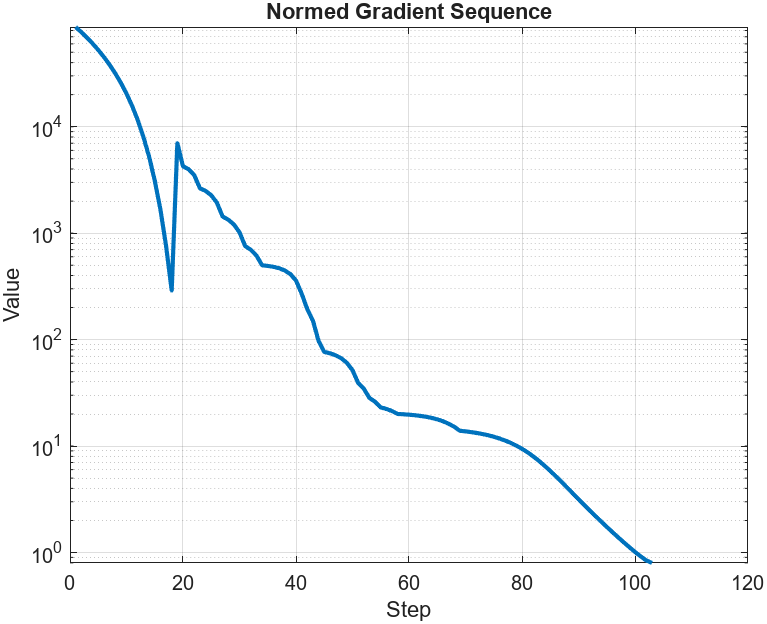
\includegraphics[width = 0.5\textwidth]{Plots/Figure_p4p1p3_NG.png}
    \caption{Dog Leg Method for initial condition described above, with $\hat{\Delta}$ = 4.25.}
    \label{fig:hw4p1p3}
\end{figure}

\newpage
\subsection{Problem 1, part 4}
 Compare NMHM (with dense linear algebra) from the previous homework and dogleg in terms of (a) number of systems solved (b) total computation time of their linear systems by starting them at the point of all 2's using the same stopping criterion for the gradient for both. Plot the two as a function of problem size for some ranges of n. Note that the n range need not be the same for both as the timings may be different. Discuss your findings and explain why the results may behave as you observe. 
 \partbreak
 \begin{solution}

     I have included the two relevant plots below. For the NMHM plot, I know there is something wrong with the normed gradient converging to zero. I can say that after a weekend's worth of debugging, that it \textit{does} converge, just not to zero. I honestly don't know why. We can see that the average time to solve the linear system is greater for Dogleg, but there are overall fewer linear systems calculated. To somehow rationalize my findings, I would say that the say that sparse matrices are stored in memory isn't contiguous, unlike the case for dense matrices. And as such, for lower dimensions as what I have here, we see this difference. PLEASE BE IN THE MATLABCODE FOLDER WHEN RUNNING ALL CODE. IF YOU ARE NOT, YOU WILL GET AN ERROR. I wanted to separate the two methods via folders, so I change the current directory when calling the two methods. 
 \end{solution}

\vspace{1cm}
 \begin{figure*}[!htb]
  \centering
  \begin{minipage}{0.4\textwidth}
    \centering
    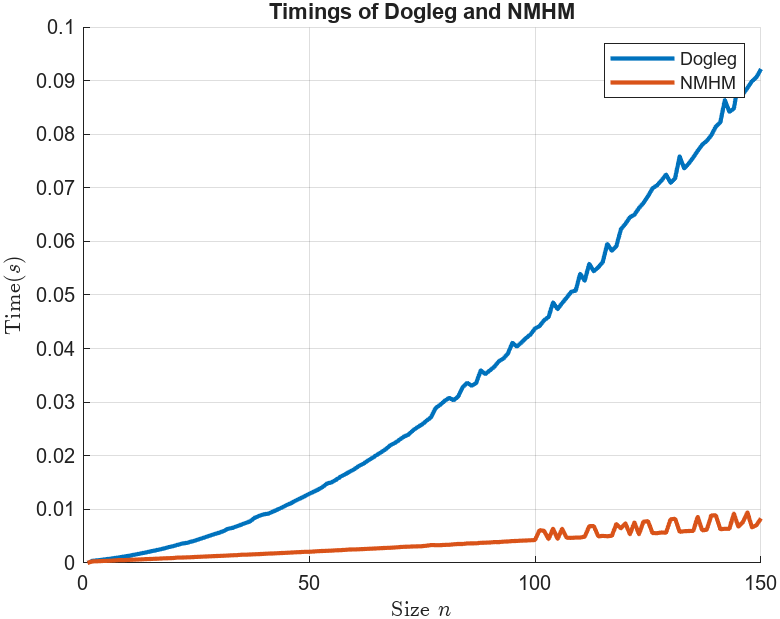
\includegraphics[width=\linewidth]{Plots/timings_diff.png}
    \caption{ The average time to solve the linear system for NMHM and Dogleg methods.}
    \label{fig:img1}
  \end{minipage}\hfill
  \begin{minipage}{0.4\textwidth}
    \centering
    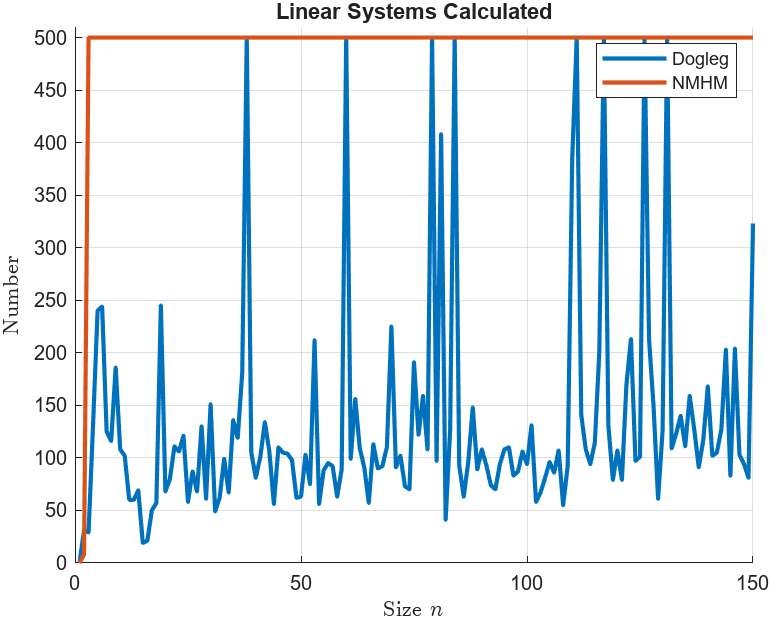
\includegraphics[width=\linewidth]{Plots/num_lin_sys.png}
    \caption{The number of linear systems calculated up to 150 dimensions.}
    \label{fig:img2}
  \end{minipage}
\end{figure*}
\newpage
\section{Problem 2}
This problem we will carry out what I mentioned in class when I realized my insight was incorrect. Assume that you try to solve the trust-region problem approximately, as I did in class with the dogleg. In other words you aim to solve the problem \\
$\min_{p} := f + g\T p + \frac{1}{2}p\T Bp, \quad \norm{p} \leq \Delta$.\\
Assume now that (a) $B$ is invertible and has at least one negative eigenvalue, (b) $p^N$ is a solution of the Newton system $Bp^N = -g$ and (c) $\norm{p^N} < \Delta$ (that is, the Newton point is interior to the trust region, the situation I was implementing in class). Prove now that there exists a direction $p^D$ such that $m(p^N + \ep p^D) < m(p^N)$ for $\ep$ sufficiently small. In other words, $p^N$ cannot be a solution of the trust region method even if it is a solution of the Newton equation.
\partbreak
\begin{solution}

    We will begin by expanding $m(p^n + \ep p^D)$
    \tightalignbreak
    \begin{align*}
        m(p^n + \ep p^D) &= f + g\T (p^N + \ep p^D) + \frac{1}{2}(p^N + \ep p^D)\T B(p^N + \ep p^D)\\
        &= f + g\T p^n + \ep g\T p^d + \frac{1}{2}\left[(p^N)\T Bp^N + \ep(p^n)\T Bp^D + \ep (p^D)\T Bp^n + \ep^2 (p^D)\T Bp^D \right]\\
        &= f + g\T p^N + \frac{1}{2} (p^N)\T Bp^N + \ep g\T p^D + \frac{1}{2}\left[ \ep((p^N)\T Bp^D + (p^D)\T Bp^N + \ep (p^D)\T Bp^D\right]\\
        &= m(p^N) + \ep \left( g\T p^D + \frac{1}{2}(p^N)\T Bp^D + \frac{1}{2}(p^D)\T Bp^N + \frac{\ep}{2}(p^D)\T Bp^D\right) 
    \end{align*}
    \vspace{-6mm} \alignbreak
    By the calculations above, we just need to show that the quantity in parenthesis can be negative for some choice of search direction $p^D$. If we show this, then we will show that $p^N$ cannot be a solution. Note that from (b) we have $Bp^N = -g$. Plugging this into the quantity in parenthesis, we have
    \[ -(p^N)\T B\T p^D + \frac{1}{2}(p^N)\T Bp^D + \frac{1}{2}(p^D)\T Bp^N + \frac{\ep}{2}(p^D)\T Bp^D\]
    By transposition, we can rewrite every suitable instance of $p^D$ being pre-multiplied by $B$. Then, 
    \[ -(p^N)\T  Bp^D + \frac{1}{2}(p^N)\T Bp^D + \frac{1}{2}(B\T p^D)\T p^N + \frac{\ep}{2}(p^D)\T Bp^D\]
    Since we have that $B$ has one negative eigenvalue, suppose that $p^D$ is the eigenvector associated with this eigenvalue. We can then write $Bp^D = -\lm p^D$, for $\lm > 0$. By the properties of linear algebra, $\lm$ is also an eigenvalue of $B\T$ since we are over the real numbers. Thus, the following can be written:\\
    \tightalignbreak
    \begin{align*}
        &-(p^N)\T B p^D + \frac{1}{2}(p^N)\T Bp^D + \frac{1}{2}(B\T p^D)\T p^N + \frac{\ep}{2}(p^D)\T Bp^D &\text{(Given.)}\\
        &-(p^N)\T (-\lm) p^D + \frac{1}{2}(p^N)\T (-\lm)p^D + \frac{1}{2}(-\lm p^D)\T p^N + \frac{\ep}{2}(p^D)\T (-\lm)p^D &(Bp^D = -\lm p^D.)\\
        &\lm (p^N)\T p^D - \frac{\lm}{2}(p^N)\T p^D - \frac{\lm}{2}(p^D)\T p^N - \frac{\lm \ep}{2}(p^D)\T p^D &\text{(Rearranging.)}\\
        &\lm (p^N)\T p^D - \frac{\lm}{2}(p^N)\T p^D - \frac{\lm}{2}(p^N)\T p^D - \frac{\lm \ep}{2}(p^D)\T p^D &\text{(Inner product symmetry.)}\\
        &= - \frac{\lm \ep}{2}(p^D)\T p^D &\text{(Cancelling.)}\\
        &= -\frac{\lm\ep}{2}\norm{p^D}^2 &\text{(Definition.)}
    \end{align*}
    \vspace{-6mm}\alignbreak
    Since $\lm,  \ep > 0$, we have that the above term is overall negative. Therefore, an additional direction $p^D$ has been obtained which minimizes the approximate solution.
\end{solution}
\newpage
\section{Problem 3}
\newcommand{\alphabar}{\overline{\alpha}}
We will show that steepest descent with backtracking has asymptotic linear convergence. Let $x_k$ be a sequence produced by steepest descent with line search and backtracking when applied to the nonlinear optimization problem $\min_{x} f(x)$, where the function $f(x)$ is three times continuously differentiable. This is the algorithm you implemented in the second homework except you will apply it to a general function. In particular, we will assume that backtracking is initialized at a fixed stepsize $\alphabar$ as we did in problem 2 in homework 2. Assume that $x_k \rightarrow x\star$ where $x\star$ satisfies the second order sufficient conditions. 

\subsection{Problem 3, part a}
Prove that there exists a neighborhood of $x\star$ and parameters $0 < c_1 < c_2$ such that $c_1 \norm{\grad f(x)}^2 \leq f(x) - f(x\star) \leq c_2\norm{\grad f(x)}^2$ for any $x$ within the neighborhood $N(x\star)$.
\partbreak

\begin{solution}

    The first inequality can be shown as follows. We first note that the neighborhood $N(x\star)$ can be chosen around $x\star$ such that $f(x \in N(x\star))$ is convex, as well as the gradient $\grad f(x)$ is Lipshchitz. Note that \cite{zhou2018fenchel} gives\footnote{This result is [5] on page 4. I have two choices concerning this: I can either give my own, sloppier version of the proof; or I can cite the reference itself. I feel it is more transparent that I cite it.}. 
    \[f(y) \geq f(x) + \grad f(x)\T (y - x) + \frac{1}{2L}\norm{\grad f(y) - f(x)}^2, \quad \forall x, y.\]
    This result is directly applicable when we restrict $x, y \in N(x\star)$, so that we can assure convevity of $f$ and Lipschitzness of $\grad f$. Substituting $y \mapsto x$ and $x \mapsto x\star$ gives,
    \[f(x) \geq f(x\star) + \grad f(x\star)\T (x - x\star) + \frac{1}{2L}\norm{\grad f(x) - \grad f(x\star)}^2.\]
    By the second order sufficient conditions, we have that $\grad f(x\star) = 0$, so we get 
    \[\frac{1}{2L}\norm{\grad f(x)}^2 \leq f(x) - f(x\star).\]
    So we have $c_1 = \frac{1}{2L}$. To find the second inequality, we can approximate the function $f(x)$ for some $x \in N(x\star)$, 
    \[f(x) = f(x\star) + \grad f(x\star)(x - x\star) + \frac{1}{2}(x - x\star)\T \grad^2 f(x\star)(x - x\star).\]
    By the second order sufficient conditions we have $\grad f(x\star) = 0$, so with rearranging, we have
    \[f(x) - f(x\star) = \frac{1}{2}(x - x\star)\T \grad^2 f(x\star)(x - x\star)\]
    The right hand side can be bounded by Cauchy Schwartz to give
    \[f(x) - f(x\star) \leq \norm{x - x\star}^2 \norm{\grad^2f(x\star)}.\]
    By problem 3 part a of Homework 2 we found 
    \[c'\norm{x - x\star} \leq \norm{\grad f(x)},\]
    for some $c' > 0.$ We can substitute this into our inequality to get
    \[f(x) - f(x\star) \leq \frac{1}{2(c')^2} \norm{\grad^2f(x\star)}\norm{\grad f(x)}^2.\]
    Therefore, setting $c_2 = \frac{1}{2(c')^2}\norm{\grad^2 f(x\star)}$, we have found the following chain of inequalities to be found.  
\end{solution}

\newpage
\subsection{Problem 3, part b}
In the case where $f(x)$ is quadratic,
$f(x) = f + g\T x + \frac{1}{2}x\T Bx,$ $ B\succ 0$ find the sharpest values of $c_1, c_2$ as a function of the eigenvalues of $B$. Prove that they are the sharpest by finding $x \neq x\star$, where the inequalities above are, in effect, equalities.
\partbreak
\begin{solution}

    For the case of the quadratic, we can take some shortcuts in the calculation of $c_1$ and $c_2$ in the previous part. Define $\psi(x) = f(x) - f$. We note that analyzing $\psi$ over $f(x)$ will return equivalent bounds. Note that 
    \[\psi(x) = \frac{1}{2}\braket{x - x\star}{B(x - x\star)} \leq \frac{\norm{B}}{2}\norm{x - x\star}^2 = \frac{\lm_{\max}}{2}\norm{x - x\star}^2.\]
    From the previous homework, we found that $\norm{x - x\star} \leq \frac{1}{\lm_{\max}^2}\norm{\grad f(x)}^2$, so substituting this in, we find 
    \[\psi(x) = f(x) - f \leq \frac{1}{2\lm_{\max}}\norm{\grad f(x)}^2.\]
    This then settles the upper bound. We can then find the lower bound in the following manner:\\

    \quad 
    DO THIS ONE.
    \quad

    We now have $c_1 = \frac{1}{2\lm_{\min}},\ c_2 = \frac{1}{2\lm_{\max}}$.
\end{solution}

\newpage
\subsection{Problem 3, part c}
Use point (a) to show that one our iteration stays in that neighborhood of $x\star$, we will have
\[f(x^{k+1}) - f(x\star) \leq ( 1 - \eta_k)(f(x^k) - f(x\star)\]
for some $\eta_k > 0$. I suggest you to start form the analysis you did at Problem 2, homework 2 and obtain $\eta_k$ from there. Note that via the iteration, we can rewrite $\norm{p_k}$ in terms of $\norm{\grad f_k}$. This is found from $x_{k+1} = x_k + \alpha_k p_k$. which can be rewritten as $\norm{p_k} \geq \norm{x_k - x\star}$. Then we can apply part a from last homework to this to get an inequality to $\norm{\grad f_k}$
\partbreak
\begin{solution}

    Note that the given inequality can be rewritten in the following form:
    \[f(x^{k+1} \leq f(x^k) + \eta^k (f(x\star) - f(x^k)\]
    From Homework 2, part 2, we were analyzing a sequence which was of the form $x^{k+1} = \alpha^k + p^k$. We will start in a similar manner as in that problem. Note I will be shorthanding $f(x^i) = f_i$. 
    \tightalignbreak
    \begin{align*}
        f_{k+1} &\leq f_k + c_1\alpha_k \grad f_k\T p_k &\text{(Start.)}\\
        &\leq f_k + c_1\rho \Bar{\alpha} \grad f_k\T p_k &\text{(Backtracking bound.)}\\
        &\leq f_k - x_1\rho\Bar{\alpha} \norm{\grad f_k\T p_k} &\text{(Norm of negative value.)}\\
        &\leq f_k - c_1 \rho\Bar{\alpha}\norm{\grad f_k} \norm{p_k} &\text{(Cauchy Schwartz.}\\
        &\leq f_k - c_1 \rho \Bar{\alpha} \norm{\grad f_k}^2 &\text{(Iteration.)}\\
        &\leq f_k - c_1 \rho\Bar{\alpha}(2\lm_{\max})(f(x_k) - f(x\star)) &\text{(From part a.)}\\
        \implies& \eta_k = 2c_1\rho\Bar{\alpha}\lm_{\max} &\text{(Comparing.)} 
    \end{align*}
    \vspace{-12mm}\alignbreak
    Note that $\lm_{\max}$ is the max eigenvalue of $B_k$, which is $\eta$'s dependence on $k$.
\end{solution}

\newpage
\subsection{Problem 3, part d}
Show now that $\eta_k$ is uniformly bounded below away from zero, and concluded that $f(x^k) - f(x\star)$ converges Q-linearly to zero.
\partbreak
\begin{solution}

    Note that $B_k$ is an approximation to the Hessian $\grad^2f(x_k)$. As $k\rightarrow \infty$, we have that $\norm{B_k} \rightarrow \norm{\grad^2f(x\star)}$. Since $x\star$ satisfies the second order sufficient conditions, we have that $\grad^2(fx\star) \succ 0$, which implies that $\lm_{\max}$ is bounded away from zero. Due to this reason, taking norms on each side of the inequality in part c, we get
    \[\norm{f_{k+1} - f(x\star)} \leq |1 - \eta_k|\norm{f_k - f(x\star)}.\]
    Dividing through by $\norm{f_k - f(x\star)}$ tells us that the ratio between function evaluations is bounded by $|1 - \eta_k|$, which we showed was bounded away from zero. Therefore, $f(x^k) - f(x\star)$ converges Q-linearly to zero.  
\end{solution}

\subsection{Problem 3, part e}
Show that the sequence $\norm{x_k - x\star}, \ \norm{\grad f(x^k)}$ converge R-linearly to zero. 
\partbreak
\begin{solution}

    To show these two sequences converge R-linearly to zero, we just need to show that there is some other sequence $r_k$ which bounds the sequence and converges Q-linearly to zero. Note that by part a, $\norm{\grad f(x)}^2$ is bounded by $\frac{1}{c_1} (f(x) - f(x\star))$. Since we showed the sequence $f(x_k) - f(x\star)$ converges Q-linearly to zero, and it bounds $\norm{\grad f(x)}^2$ for any $x$ in our neighborhood of $x\star$, then $\norm{\grad f(x_k)}$ converges R-linearly to zero. Doing the same procedure with the relationship we found between $\norm{x - x\star}$ and $\norm{\grad f(x)}$ in Homework 2, Problem 3, we have that $\norm{x^k - x\star}$ converges R-linearly to zero. Note that we are free to apply this result from problem 3, since we satisfy the same conditions. 
\end{solution}

\newpage
\subsection{Problem 3, part f}
Is it possible for the convergence rate to be quadratic?
\partbreak
\begin{solution}

    Note that we are only using information about the gradient, not the Hessian. Only Newton's method converges quadratically, which requires the exact hessian of the function to work. Thus, we are only guaranteed at most superlinear convergence.  
\end{solution}
\end{document}